\documentclass[fleqn]{article}
\usepackage{graphicx}
\usepackage{polski}
\usepackage[utf8]{inputenc}
\usepackage{listings}
\usepackage{amsmath}
\usepackage{courier}
\usepackage[top=0.3in, bottom=0.8in, left=0.8in, right=0.8in, a5paper]{geometry}
\newcommand\numberthis{\addtocounter{equation}{1}\tag{\theequation}}
\renewcommand{\familydefault}{\sfdefault}

\usepackage{listings}
\usepackage{color}
 
\definecolor{codegreen}{rgb}{0,0.6,0}
\definecolor{codegray}{rgb}{0.5,0.5,0.5}
\definecolor{codepurple}{rgb}{0.58,0,0.82}
\definecolor{backcolour}{rgb}{0.95,0.95,0.92}
 
\lstdefinestyle{mystyle}{
    commentstyle=\color{codegreen},
    keywordstyle=\color{magenta},
    numberstyle=\tiny\color{codegreen},
    stringstyle=\color{codepurple},
    basicstyle=\footnotesize,
    breakatwhitespace=false,         
    breaklines=true,                 
    captionpos=b,                    
    keepspaces=true,                 
    numbers=left,                    
    numbersep=5pt,                  
    showspaces=false,                
    showstringspaces=false,
    postbreak=\raisebox{0ex}[0ex][0ex]{\ensuremath{\color{red}\hookrightarrow\space}},
    showtabs=false,                  
    tabsize=2
}
\lstset{style=mystyle}

% \usepackage{color}
% \color{white}
% \pagecolor{black}

\begin{document}

\title{Symulacja ruchu N-ciał}
\author{Szymon Bugaj, Lei Peng}

\maketitle

\begin{abstract}
Sprawozdanie z projektu z przedmiotu RIM.
Tematem projektu jest symulacja ruchu N-ciał 
(N punktów materialnych pod działaniem siły grawitacji).
\end{abstract}

\tableofcontents



\section{Wstęp teoretyczny}
Projekt stanowi symulacja i wizualizacja praw fizyki klasycznej newtonowskiej. Szczególnie 3 praw dynamiki Newtona oraz siły grawitacji pomiędzy zbiorem N punktów materialnych.

Newtonowska siła grawitacji pomiędzy dwoma punktami materialnymi:
\begin{align*}
    &\vec{F_{G}} = G\frac{m_{1} m_{2}}{\|r\|^{2}}\frac{\vec{r}}{\|r\|} \\
\end{align*}

W fizyce klasycznej zależnością łączącą masę przyśpieszenie i siłę działającą na ciało jest:
\begin{align*}
    &\vec{F} = \vec{a}m \\
\end{align*}

Związek między położeniem, prędkością a przyśpieszeniem jest następujący:
\begin{align*}
    &v(t) = \frac{dp(t)}{dt} \\
    &a(t) = \frac{dv(t)}{dt} \\
\end{align*}

Mając dane położenia wszystkich N cząstek oraz ich prędkości dla danego momentu,
korzystając z powyższych równań możemy obliczyć położenie dla dowolnego punktu w dowolnym innym momencie.

\section{Rozkładanie siły grawitacji na składowe względem osi współrzędnych}
W przypadku 2D należy rozpatrzyć prostokąt o bokach równoległych do osi X i Y, gdzie w przeciwległych
wierzchołkach leżą dwa rozpatrywane ciała.

\begin{frame}
\frametitle{Rozkład wektora siły na składowe}
\begin{center}
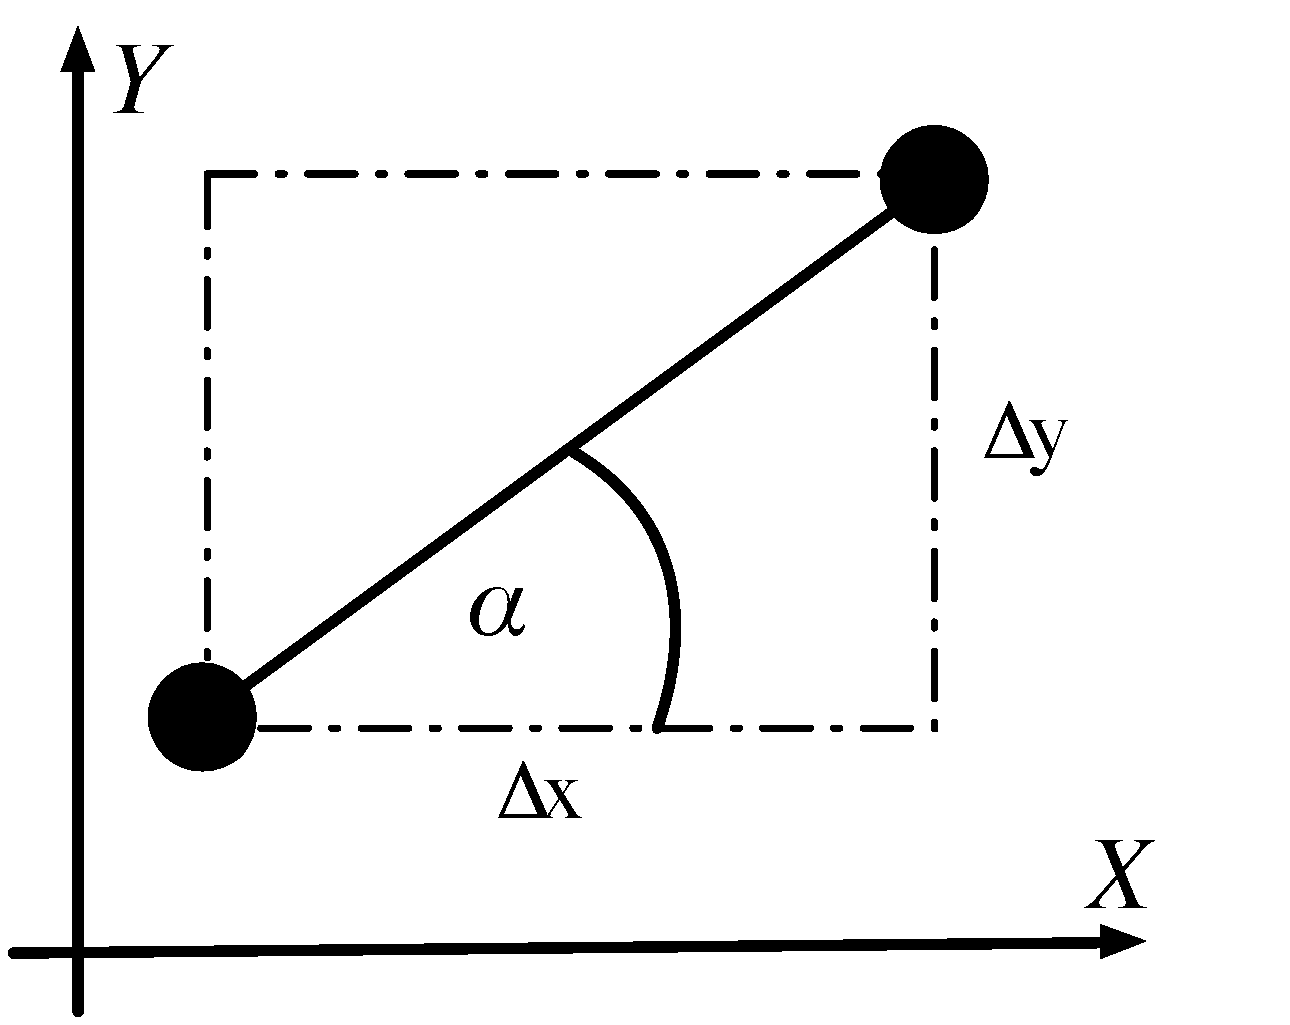
\includegraphics[width=8cm]{rozkladsil.pdf}
\end{center}
\end{frame}

\begin{align*}
    &a_{x}(t) = sin\alpha * a \\
    &a_{y}(t) = cos\alpha * a \\
\end{align*}

Dla przypadku 3D należy rozpatrzyć w analogiczny sposób prostopadłościan (ciała powinny znajdować się w wierzchołkach po przeciwnych ścianach, po przeciwnych rogach).

\section{Model numeryczny}
Interesują nas położenia ciał w kolejnych dyskretnych punktach czasu. Przyjmujemy, że w przeciągu jednostki czasu wielkości prękość, przyśpieszenie są stałe. Aktualizujemy interesujące nas wielkości w kolejności:
\begin{itemize}
    \item 1) aktualizacja prędkości
    \item 2) aktualizacja położenia
    \item 3) aktualizacja przyśpieszenia
\end{itemize}

Co należy podkreślić, wynika z tego, iż do aktualizacji prędkości brana jest poprzednia wartość przyśpieszenia.

Poniżej główna funkcja step, aktualizująca położenie, prędkość i przyśpieszenie wszystkich cząstek (NBodiesSystem.h/cpp).

% \begin{minipage}{\linewidth}
\begin {lstlisting}[language=C++]
void NBodiesSystem::step( time_type delta_t ) {
    p_prev = p_curr;
    v_prev = v_curr;

    /*
        UPDATE v SPEED and p POSITION
    */

    for (int d = 0; d < D; ++d)
        for (int i = 0; i < N; ++i) {
            v_curr.setVal(d, i, 
                v_prev.getVal(d, i)  +  
                a.getVal(d, i) * delta_t);
            p_curr.setVal(d, i, 
                p_prev.getVal(d, i)  +  
                    (v_prev.getVal(d, i) + 
                    v_curr.getVal(d, i)) 
                        * 0.5 * delta_t);
        }
    
    /*
        UPDATE a ACCELERATION
        For each two bodies i,j where i != j;
    */

    for (int d = 0; d < D; ++d)
        for (int i = 0; i < N; ++i)
            a.setVal(d, i, 0.0f);

    for (int i = 0; i < N; ++i) {
        for (int j = 0; j < N; ++j) {
            if ( i == j ) continue;

            /*
                delta X, delta Y, delta Z   
            */
            position_type* r_axis = new position_type[D];
            
            position_type r_squared = 0;
            for (int d = 0; d < D; ++d) {
                r_axis[d] = (p_curr.getVal(d, i) - 
                    p_curr.getVal(d, j));
                r_squared += r_axis[d] * r_axis[d];
            }

            position_type a_scalar = 
                G * m.getVal(0, j) / 
                pow(r_squared + efactor, 1.5);

            for (int d = 0; d < D; ++d) {
                /*
                    If both objects positions are 
                    the same there is division 
                    by zero; what to do then?
                    I just set acceleration to 0;
                */
                if (r_axis[d]) {
                    a.setVal(d, i, 
                        a.getVal(d,i) - 
                            a_scalar * 
                            (r_axis[d]/sqrt(r_squared)));
                }   
            }

            delete [] r_axis;
        }
    }
} 
\end{lstlisting}
% \end{minipage}

\section{Implementacja GPU}
By uniknąć kopiowania danych pamięć na GPU jest współdzielona przez OpenGL i CUDA. 
Funkcje zadeklarowane w cuda\_gl\_interop.h pozwalają na to: cudaGraphicsMapResources, cudaGraphicsResourceGetMappedPointer, cudaGraphicsUnmapResources (NBodiesSystemCUDA.cu).

Implementacja na GPU jest najprostszym przeniesiem kodu działającego na CPU.

\end{document}